\documentclass{article}
\usepackage[a4paper, total={6in, 8in}]{geometry}
\usepackage{graphicx}
\usepackage{float}
\usepackage{hyperref}




\usepackage{polski}
\usepackage[utf8]{inputenc}
\begin{document}


\title{Laboratorium Rozpoznawania Obrazów – Ćwiczenie \#2 Klasyfikacja optymalna Bayesa}

\author{Michał Sypetkowski}
\maketitle


\section{Dane}
Rozpatrujemy zbiór obrazów kart reprezentowanych przez niezmienniki momentowe.
Jest 8 klas, za równo w zbiorze trenującym i testującym jest wstępnie po 228 próbek na każdą klasę.

\section{Filtrowanie wartości odstających}
Algorytm filtrowania działa na danych znormalizowanych.
Dane są filtrowane poprzez odrzucenie próbek,
których wartość którejkolwiek cechy jest mniejsza
od kwartyla w 0.25 lub większa od kwartyla w 0.75 o 90 krotność odległości pomiędzy tymi kwartylami.
Implementacja jest w pliku \texttt{filter\_outliers.m}.

Ze zbioru trenującego odrzucona została próbka:
\begin{verbatim}
3.0000e+00 5.1213e+00 2.5823e+01 3.8214e+02 3.8086e+02 1.4530e+05 1.9341e+03 1.6570e+01
\end{verbatim}

Ze zbioru testującego próbki:
\begin{verbatim}
3.0000e+00 1.4815e-01 5.4870e-03 2.5403e-03 1.0161e-04 -5.1623e-08 -7.5267e-06 -1.7798e-16
3.0000e+00 1.4815e-01 5.4870e-03 2.5403e-03 1.0161e-04 -5.1623e-08 -7.5267e-06 -4.9372e-16
\end{verbatim}





\section{Optymalny klasyfikator Bayesa na 2 cechach}
Przyglądając się wizualizacji (rysunek \ref{fig:2D}) można dostrzec, że kolumny 2 i 4 (kolumna 1 to klasa) zapewniają dość dobre oddzielenie próbek różnych klas.
\begin{figure}[h]
    \caption[]{Wizualizacje 2D próbek zbioru uczącego dla wszystkich par cech}
    \centering
    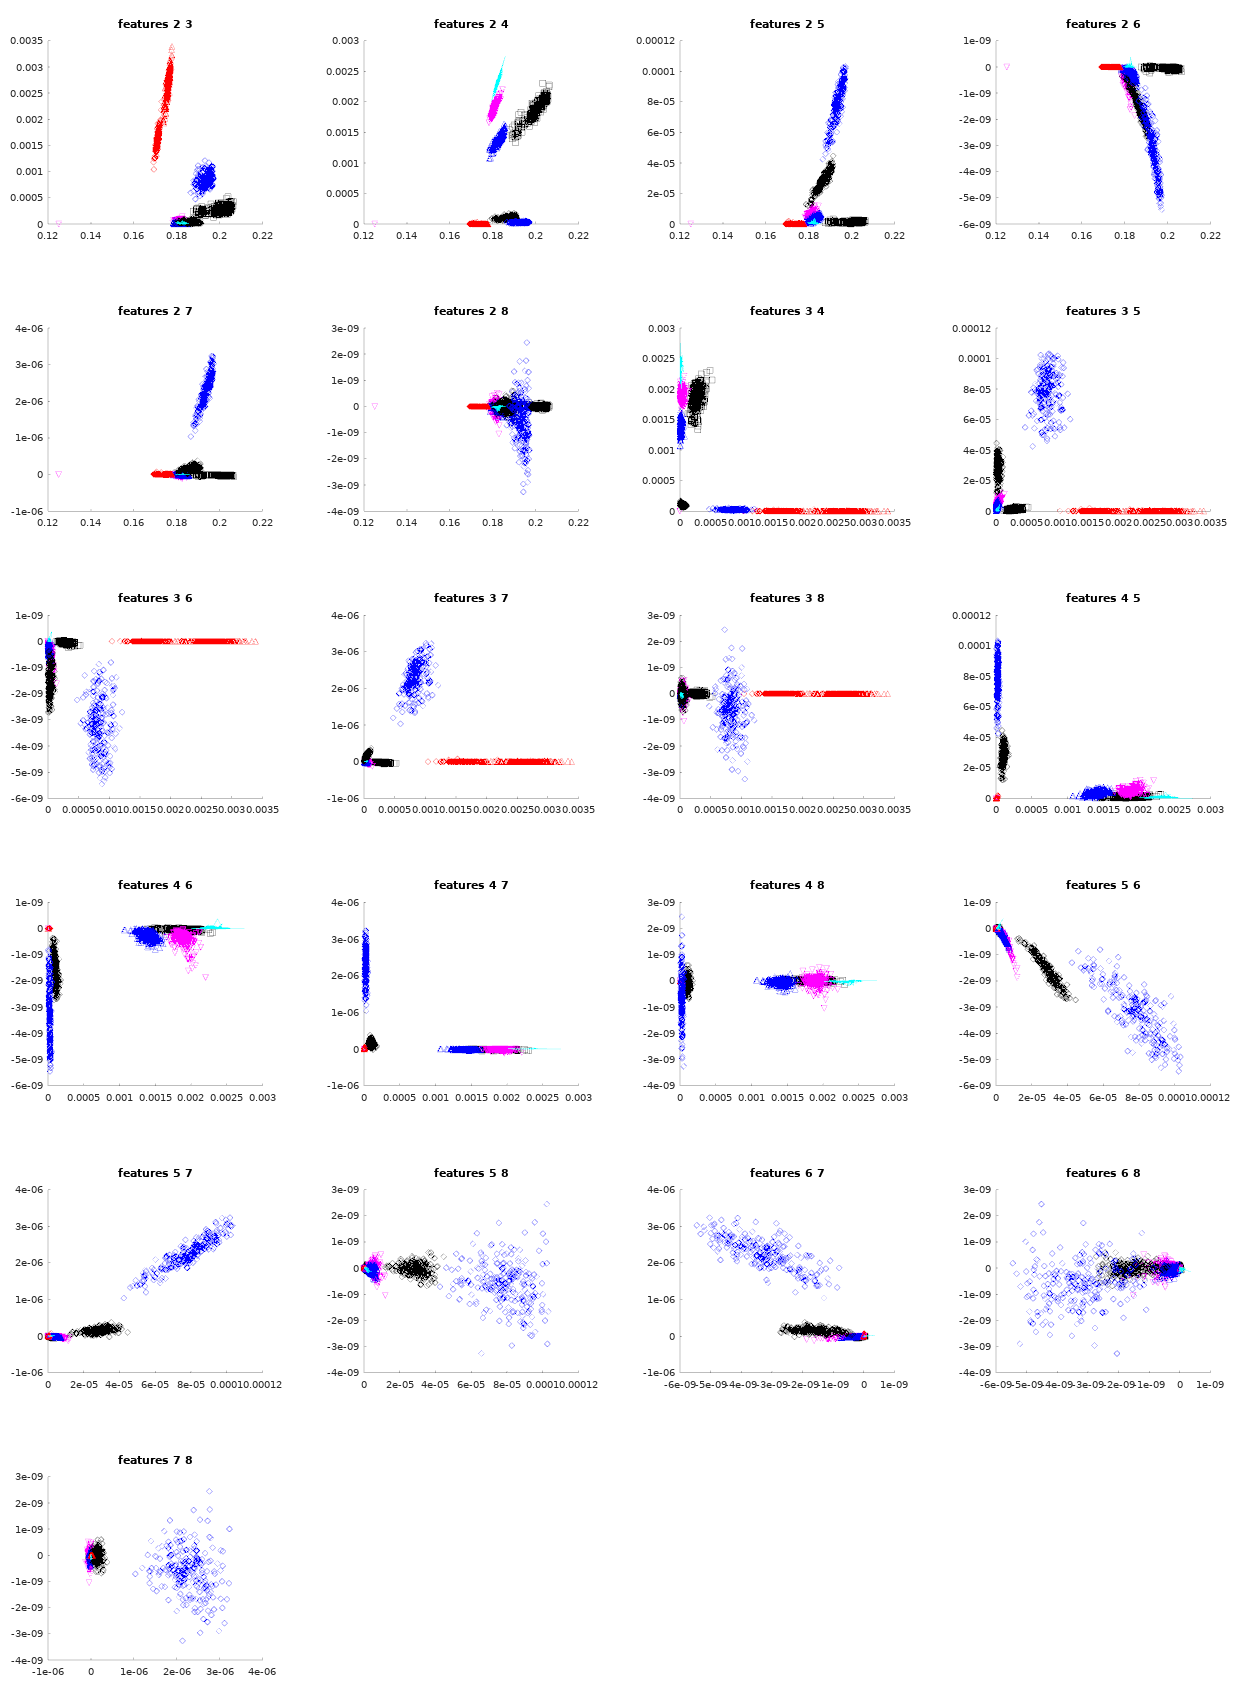
\includegraphics[width=1.0\textwidth]{2features.png}
    \label{fig:2D}
\end{figure}

\section{Wpływ doboru próbek w zbiorze uczącym na jakość klasyfikacji}
TODO
\section{Wpływ szerokości okna Parzena}
TODO
\section{Eksperyment ze zmienionym prawdopodobieństwem a priori}
TODO
\section{Porównanie z klasyfikatorem 1-NN}
TODO


\end{document}
